%auto-ignore
\chapter{Disease Knowledge Transfer across Neurodegenerative Diseases}
\label{chapter:dkt}

\newcommand{\expFld}{./jointModellingDisease/resfiles/tad-drcTiny_JMD}
\newcommand{\jmdFld}{./jointModellingDisease}


\section{Contributions}

In this chapter I present Disease Knowledge Transfer (DKT), a novel method for transferring biomarker information between related neurodegenerative diseases. I performed the mathematical modelling, implementation of the DKT method, data pre-processing, statistical analysis and model validation. The TADPOLE dataset has been assembled by myself and Neil Oxtoby, with suggestions from the EuroPOND team. The PCA dataset was acquired by the Dementia Research Centre, UK. 

While the original DKT implementation relied on a non-parametric GP disease progression model by Marco Lorenzi \cite{lorenzi2017disease} as a building block, for this thesis I chose a simpler parametric model, due to the complexity of fitting hierarchical, non-parametric, latent-space models.

\section{Publications}
\begin{itemize}
 \item R. V. Marinescu, M. Lorenzi, S. B. Blumberg, P. Planell-Morell, A. L. Young, N. P. Oxtoby,  A. Eshaghi, K. X. X. Yong, S. Crutch, D. C. Alexander, arXiv, 2019.
\end{itemize}


\section{Introduction}
\label{sec:dktInt}

The estimation of accurate biomarker signatures in Alzheimer's disease (AD) and related neurodegenerative diseases is crucial for understanding underlying disease mechanisms, predicting subjects' progressions, and selecting the right subjects in clinical trials. As a result, data-driven disease progression models (chapter \ref{chapter:bckDpm}) were proposed that reconstruct long term biomarker signatures from collections of short term individual measurements. When applied to large datasets of typical AD, disease progression models have shown important benefits in understanding the earliest events in the Alzheimer's disease cascade \cite{iturria2016early, young2014data}, the heterogeneity of AD \cite{young2018uncovering}, helped discover novel genes involved in AD \cite{scelsi2018genetic} and they showed improved predictions over standard approaches \cite{oxtoby2018}. However, by necessity these models require large datasets -- in addition they must be both multimodal and longitudinal. Such data is not available in rare neurodegenerative diseases. In particular, most datasets for rare neurodegenerative diseases come from local clinical centres, are unimodal (e.g. MRI only) and limited both cross-sectionally and longitudinally -- this makes the application of disease progression models extremely difficult.  Moreover, such a model estimated from common diseases such as typical AD may not generalise to specific variants. For example, in Posterior Cortical Atrophy -- a neurodegenerative syndrome causing visual disruption -- posterior regions such as the occipital lobe and superior parietal regions are affected early, instead of the hippocampus and temporal regions that are affected early in typical AD. 

The problem of limited data in medical imaging has so far been addressed through transfer learning methods. Such techniques have been successfully used to improve the accuracy of AD diagnosis \cite{hon2017towards, cheng2017multi} or prediction of MCI conversion \cite{cheng2015domain}, but have two key limitations. First, they use deep learning or other machine learning methods, which are not interpretable and don't allow us to understand underlying disease mechanisms that are either specific to rare diseases, or shared across related diseases. Secondly, these models cannot be used to forecast the future evolution of subjects at risk of dementia, which is important for selecting the right subjects in clinical trials. 

We propose Disease Knowledge Transfer (DKT), a generative joint model that estimates continuous multimodal biomarker progressions for multiple neurodegenerative diseases simultaneously -- including rare neurodegenerative diseases -- and which inherently performs transfer learning between the modelled phenotypes. This is achieved by exploiting biomarker relationships that are shared across diseases, whilst accounting for differences in the spatial distribution of brain pathology. DKT is interpretable, which allows us to understand underlying disease mechanisms, and can also predict the future evolution of subjects at risk of diseases. We apply DKT on Alzheimer's variants and demonstrate its ability to predict non-MRI trajectories for patients with Posterior Cortical Atrophy, in lack of such data. This is done by fitting DKT to two datasets simultaneously: (1) the TADPOLE Challenge \cite{marinescu2018tadpole} dataset containing subjects from the Alzheimer's Disease Neuroimaging Initiative (ADNI) with MRI, FDG-PET, DTI, AV45 and AV1451 scans and (2) MRI scans from patients with Posterior Cortical Atrophy from the Dementia Research Centre (DRC), UK. We first show that the estimated non-MRI trajectories for PCA subjects are plausible as they agree with previous literature findings. We finally validate DKT on three datasets: 1) simulated data with known ground truth, 2) TADPOLE sub-populations with different progressions and 3) 20 DTI scans from controls and PCA patients from the DRC, showing it yields favourable performance compared to standard approaches. Code for DKT is available online: \url{https://github.com/mrazvan22/dkt}.


\begin{figure}[h]
 \centering
 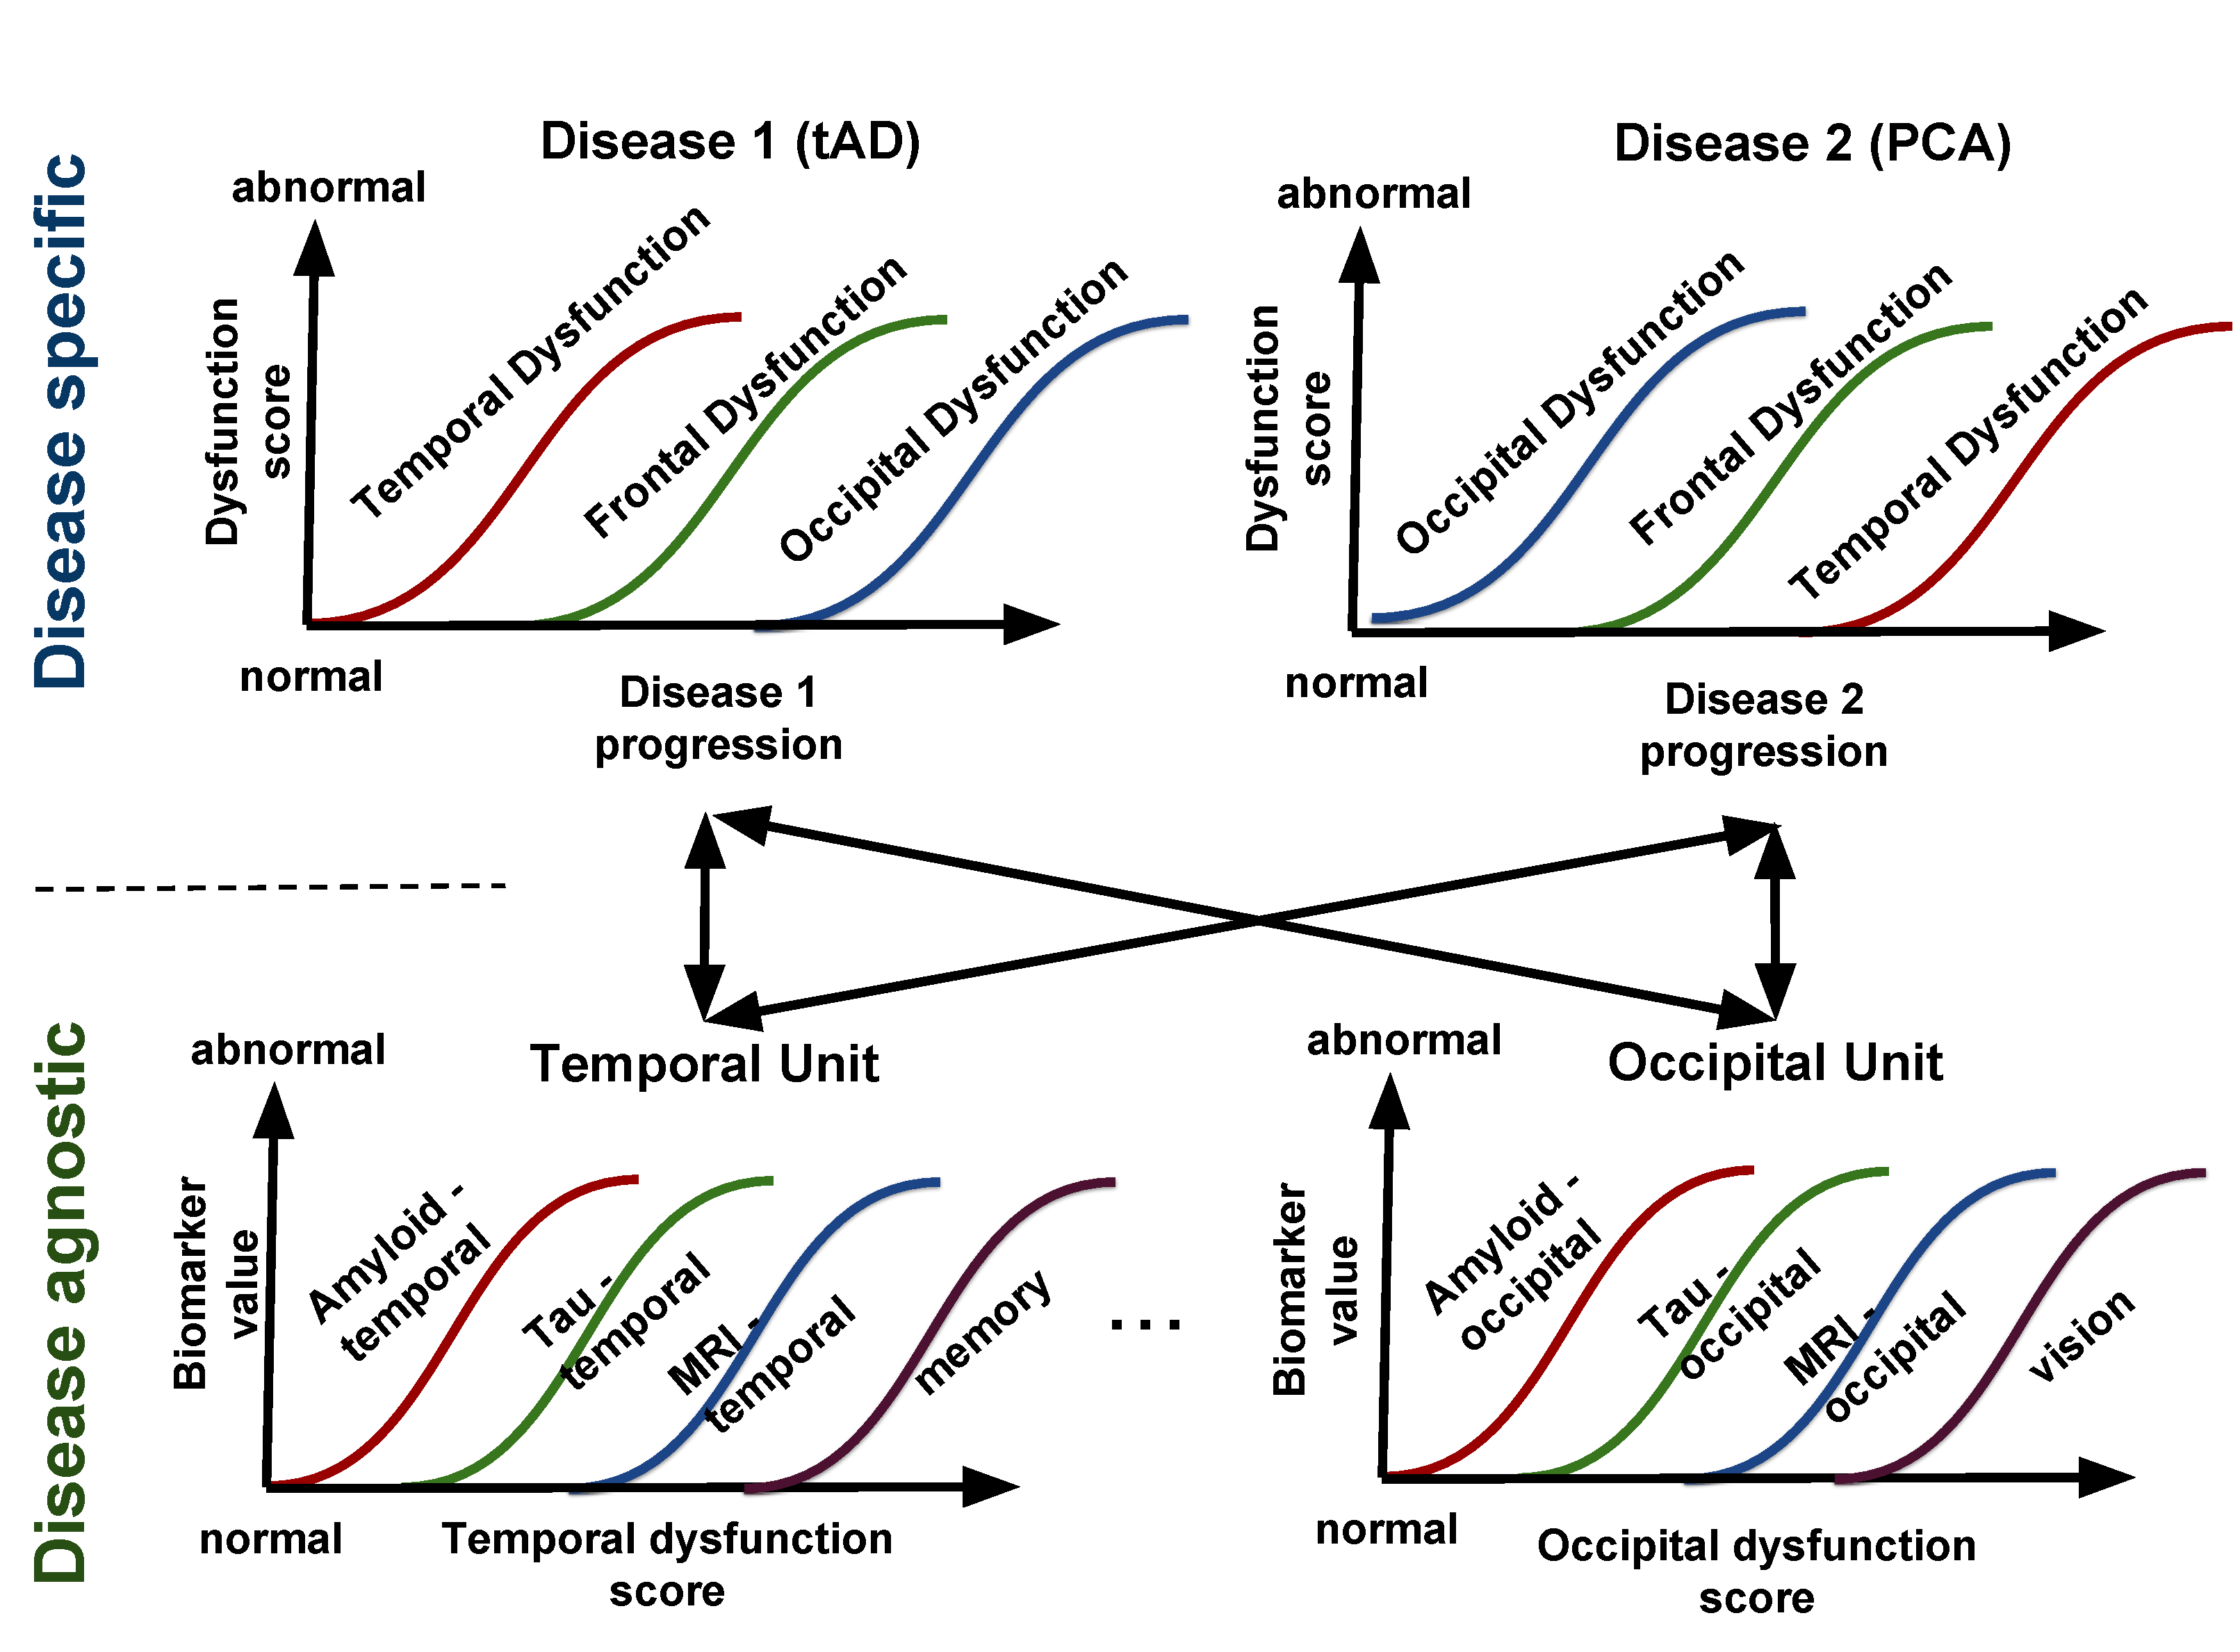
\includegraphics[width=1\textwidth,trim=0 0 0 0,clip]{\jmdFld/paper/figures/disease_knowledge_transfer.pdf}
 \caption[Diagram of the proposed framework for joint modelling of multiple diseases.]{Diagram of the proposed framework for joint modelling of multiple diseases. We assume that each disease can be modelled as the evolution of abstract dysfunctionality scores (Y-axis, top row), each one related to different brain regions. Each region-specific dysfunctionality score then further models (X-axis, bottom row) the progression of several modality-specific biomarkers within that same region. For instance, the temporal dysfunction, modelled as a biomarker in the disease specific model (top row), is the X-axis in the disease agnostic model (temporal unit, bottom row), which aggregates together abnormality from amyloid, tau and MR imaging within the temporal lobe. The biomarker correlations within the bottom units are assumed to be disease agnostic and shared across all diseases modelled. Disease knowledge transfer can then be achieved via the disease-agnostic units.}
 \label{fig:diagram}
\end{figure}

\section{Methods}
\label{sec:dktMet}


\subsection{DKT Framework}
\label{sec:dktMethFramework}
\newcommand{\lp}{\lambda_{d_i}^{\psi(k)}}
\newcommand{\lpuu}{\lambda_{d_i}^{\psi(k),(u)}}
\newcommand{\lpum}{\lambda_{d_i}^{\psi(k),(u-1)}}


Fig. \ref{fig:diagram} shows the overall diagram of our proposed framework for joint modelling of diseases. We assume that the progression of each disease (X-axis, top row) can be modelled as the evolution of abstract dysfunctionality scores, each one related to different brain regions (top row). Each dysfunctionality score is then modelled as the progression of several biomarkers within that same region, but acquired using different noninvasive imaging modalities (bottom row). Each group of biomarkers in the bottom row will be called a \emph{functional unit}, because the correlations between biomarkers are related through common "function" in a disease--agnostic way, since they are related to the same underlying brain region. Biomarker groupings into functional units are defined a-priori. We choose to model the correlations within each unit using the disease progression model (DPM) by Jedynak et al. \cite{jedynak2012computational}, but any other DPM can also be used. The DPM allows us to reconstruct unit-specific \emph{dysfunction} progression manifolds (bottom row, X axis), which can be used for staging subjects. Finally, we use the same DPM to express the progression within each disease (Figure 1, top) in terms of the dysfunction scores estimated within each functional unit. More precisely, the X-axis dysfunction scores from the functional units become Y-axis measurements in the disease specific models.

The model has a concise mathematical formulation. We assume a set of given biomarkers measurements $Y = [y_{ijk} | (i,j,k) \in \Omega]$ for subject $i$ at visit $j$ in biomarker $k$, where $\Omega$ is defined as the set of available biomarker measurements, since subjects can have missing data at various visits. We assume that each subject $i$ at each visit $j$ has an underlying disease stage $s_{ij} = \beta_i + m_{ij}$, where $m_{ij}$ represents the months since baseline visit for subject $i$ at visit $j$ and $\beta_i$ represents the time shift of subject $i$. We further denote by $\theta_k$ the parameters used to represent the trajectory for biomarker $k \in K$ within its functional unit $\psi(k)$, where $\psi$: \{1, ..., K\} $ \rightarrow \Lambda$ is a function that maps each biomarker $k$ to a unique functional unit $l \in \Lambda$, where $\Lambda$ is the set of functional units. Moreover, we denote by $\lambda_d^l$ the parameters for the trajectory of the dysfunction score corresponding to functional unit $l \in \Lambda$ in the space of disease $d$. These definitions allow us to formulate the likelihood for a single measurement $y_{ijk}$ as follows:

\begin{equation}
 p(y_{ijk}|\theta_k, \lp, \beta_i, \epsilon_k) = N(y_{ijk}| g(f(\beta_i + m_{ij}); \lp; \theta_k), \epsilon_k)
\end{equation}
where $g(\ .\ ; \theta_k)$ represents the trajectory of biomarker $k$ within functional unit $\psi(k)$ and $f(\ .\ ; \lambda_{d_i}^{\psi(k)})$ represents the trajectory of the functional unit $\psi(k)$ within the space of disease $d_i$. To be precise, $d_i \in \mathbb{D}$ represents the index of the disease space where subject $i$ belongs, where $\mathbb{D}$ is the set of all diseases modelled. For example, MCI and tAD subjects from ADNI as well as tAD subjects from the DRC cohort can all be assigned $d_i=1$, while PCA subjects from the DRC dataset can be assigned $d_i=2$. Healthy controls can be assigned to either disease space, although a more precise assignment would take molecular biomarkers into account. Variable $\epsilon_k$ denotes the variance of measurements for biomarker $k$. 

We extend the above model to multiple subjects, visits and biomarkers to get the full model likelihood:
\begin{equation}
 p(\boldsymbol{y}|\theta, \lambda, \beta , \epsilon) = \\ \prod_{(i,j,k) \in \Omega} p(y_{ijk}|\theta_k, \lp, \beta_i) 
\end{equation}

where $\boldsymbol{y} = [y_{ijk} | \forall (i,j,k) \in \Omega ]$ is the vector of all biomarker measurements, while $\boldsymbol{\theta} = [\theta_1, ..., \theta_K]$ represents the stacked parameters for the trajectories of biomarkers in functional units, $\boldsymbol{\lambda} = [\lambda_d^{l}|l \in \Lambda, d \in \mathbb{D}]$ are the parameters of the dysfunctionality trajectories within the disease models, $\boldsymbol{\beta} =[\beta_1, ..., \beta_N]$ are the subject-specific time shifts and $\boldsymbol{\epsilon} = [\epsilon_k | k \in K]$  estimates biomarker measurement noise. Although we assumed independence across different subjects, biomarker measurements and visits are linked using the latent time-shift $\beta_i$ for each subject. The parameters of the model that need to be estimated are $[\boldsymbol{\theta}, \boldsymbol{\lambda}, \boldsymbol{\beta}, \boldsymbol{\epsilon}]$. For model simplicity, we did not account for inter-individual variability other than that expressed by the time-shift $\beta_i$, although this could be extended in future work.

\subsection{Modelling Biomarker Trajectories}
\label{sec:dktBiomkTraj}

So far we defined the DKT framework using generic models $g(\ .\ ; \theta_k)$ and $f(\ .\ ; \lp)$ for the biomarker trajectories within the functional units and the disease models. Now we choose to implement the $f$ and $g$ models as parametric sigmoidal curves, to enable a robust optimisation and because these models account for the floor and ceiling effects normally observed in AD biomarkers \cite{sabuncu2011dynamics,caroli2010dynamics}. The sigmoidal model for $f$ is defined as:

\begin{equation}
 f(s;\theta_k) = \frac{a_k}{1+exp(-b_k(s-c_k))} + d_k
\end{equation}

where $s$ is the disease progression score of a subject and $\theta_k = [a_k, b_k, c_k, d_k]$ are parameters controlling the shape of the trajectory for biomarker $k$: $d_k$ and $d_k + a_k$ represent the lower and upper limits of the sigmoidal function, $c_k$ represents the inflection point and $a_k b_k/4$ represents the slope at the inflection point. A similar model is used also for $g$. 

\subsection{Parameter Estimation}

\newcommand{\uu}{^{(u)}}
\newcommand{\um}{^{(u-1)}}


We estimate the model parameters using a two-stage approach. In the first stage, we perform belief propagation within each functional unit and then within each disease model. Each functional unit and disease model is assumed to be an independent disease progression model that we fit by alternatively optimising the fit of biomarker trajectories and subject-specific time-shifts, using the approach described in \cite{jedynak2012computational}. At this stage we assume the existence of a latent variable $\beta_i^{\psi(k)} = f(\beta_i + m_{ij}; \lp)$ representing the dysfunctionality score of subject $i$ within the functional unit $\psi(k)$, which represents a time-shift within that functional unit.

In the second stage we jointly optimise across all functional units and disease models using loopy belief propagation. An overview of the algorithm is given in Figure \ref{fig:dktAlgo}. Given the initial parameters estimated from the first stage (line 1), the algorithm continuously updates the biomarker trajectories within the functional units (lines 4-5), dysfunctionality trajectories (line 9) and subject-specific time shifts (line 13) until convergence. The cost function for all parameters is nearly identical, the main difference being the measurements $(i,j,k)$ over subjects $i$, visits $j$ and biomarkers $k$ that are selected for computing the measurement error. For estimating the trajectory of biomarker $k$ within functional unit $\psi(k)$, measurements are taken from $\Omega_k$ representing all measurements of biomarker $k$ from all subjects and visits. For estimating the dysfunctionality trajectories,  $\Omega_{d,l}$ represents the measurement indices from all subjects with disease $d$ (i.e. $d_i = d$) and all biomarkers $k$ that belong to functional unit $l$ (i.e. $\psi(k) = l$). Finally, $\Omega_i$ (line 13) represents all measurements from subject $i$, for all biomarkers and visits. 

The algorithm we proposed in Figure \ref{fig:dktAlgo} has a complexity of $O(I*S)$, where $S$ is the number of subjects in the dataset and $I$ is the number of iterations until convergence. In practice, convergence is achieved after around 10-15 iterations, which takes around 1h on a Xeon CPU E5-2680 @ 2.5GHz.


\begin{figure}
\begin{algorithm}[H]
 Initialise $\boldsymbol{\theta}^{(0)}$, $\boldsymbol{\lambda}^{(0)}$, $\boldsymbol{\beta}^{(0)}$\\
  \While{$\boldsymbol{\theta}$, $\boldsymbol{\lambda}$, $\boldsymbol{\beta}$ not converged}{
   \tcp*[l]{Estimate biomarker trajectories (disease agnostic)}
    \For{$k=1$ to $K$}{
      ${\theta_k\uu = \argmin_{\theta_k} \sum_{(i,j) \in \Omega_k} \left[y_{ijk} - g\left(f(\beta_i\um + m_{ij}; \lpum) ; \theta_k\right) \right]^2  - log\ p(\theta_k)}$\\
      ${\epsilon_k\uu = \frac{1}{|\Omega_k|} \sum_{(i,j) \in \Omega_k}    \left[y_{ijk} - g\left(f(\beta_i\um + m_{ij}; \lpum) ; \theta_k\uu \right) \right]^2 }$\\
    }
     \tcp*[l]{Estimate dysfunctionality trajectories (disease specific)} 
    \For{$d=1 \in \mathbb{D}$}{
      \For{$l=1 \in \Lambda$}{
        ${\lambda_{d}^{l, (u)} = \argmin_{\lambda_{d}^{l}} \sum_{(i,j,k) \in \Omega_{d,l}} \left[y_{ijk} - g\left(f(\beta_i\um + m_{ij}; \lambda_{d}^{l}) ; \theta_k\uu 
        \right) \right]^2  - log\ p(\lambda_{d}^{l})}$\\
      }
    }
    \tcp*[l]{Estimate subject-specific time shifts} 
    \For{$i=1 \in [1, \dots, S]$}{
      ${\beta_i\uu = \argmin_{\beta_i} \sum_{(j,k) \in \Omega_i} \left[y_{ijk} - g\left(f(\beta_i + m_{ij}; \lpuu) ; \theta_k\uu
      \right) \right]^2  - log\ p(\beta_i)}$\\
    }
}
\end{algorithm}
\caption[The algorithm for estimating the DKT parameters]{The algorithm for estimating the DKT parameters. The algorithm successively updates the biomarker trajectories within the functional units (disease agnostic models), dysfunctionality trajectories (disease specific) and subject-specific time shifts until convergence.}
\label{fig:dktAlgo}
\end{figure}

\subsection{Synthetic Experiment}
\label{sec:dktMetSyn}

We first test DKT on synthetic data, in order to assess the performance when ground truth is known. We generate synthetic data from two diseases as follows:
\begin{itemize}
 \item[] \textbf{Disease model}
 \item We define two functional units $l_0$ and $l_1$ and 6 biomarkers $k_0-k_5$, which we allocate to functional units as follows: $l_0:\{k_0, k_2, k_4\}$, $l_1: \{k_1, k_3, k_5\}$. Within their units, we define the trajectory of each biomarker as a sigmoidal curves with the following $\theta_k$ parameters:
 \begin{itemize}
  \item functional unit $l_0$: $\theta_0 = (1,5,0.2,0)$, $\theta_2 = (1,5,0.55,0)$ and $\theta_4 = (1,5,0.9,0)$ 
  \item functional unit $l_1$: $\theta_1 = (1,10,0.2,0)$, $\theta_3 = (1,10,0.55,0)$ and $\theta_5 = (1,10,0.9,0)$ 
 \end{itemize}
 \item We define two synthetic diseases, "synthetic AD" ($d=0$) and "synthetic PCA" ($d=1$). For each disease $d$, each functional unit $l$ has a distinct dysfunctionality trajectory defined as a sigmoidal curve with parameters $\lambda_d^l$ as follows: 
 \begin{itemize}
  \item "synthetic AD" disease: $\lambda_0^0 = (1, 0.3, -4, 0)$  and $\lambda_0^1 = (1, 0.2, 6, 0)$.
  \item "synthetic PCA" disease: $\lambda_1^0 = (1, 0.3, 6, 0)$ and $\lambda_1^1 = (1, 0.2, -4, 0)$.
 \end{itemize}

 \item[] \textbf{Subject model}
 \item We generated time-shifts $\beta_i$ for 100 subjects (disease $d_0$) and 50 subjects (disease $d_1$) based on a uniform distribution with ranges $(-13, 10)$ years before/after disease onset. 
 \item Within each disease, we generated the subjects' diagnosis (controls/patients) based on an exponential likelihood model with mean -4.5 (controls)/4.5 (patients) years before/after disease onset. 
 \item For each subject and each biomarker, we generated data for four consecutive visits, each visit one year apart, using a noise standard deviation of 0.05.
\end{itemize}

These trajectory and subject parameters were chosen to mimic the TADPOLE and DRC cohorts, described below. Before fitting DKT on the synthetic dataset, we discarded the data from biomarkers $k_0$, $k_1$, $k_4$ and $k_5$ for all subjects within the synthetic PCA cohort, to simulate the lack of multimodal data in these subjects. Remaining biomarkers $k_2$ and $k_3$, for which data was still available in the synthetic PCA cohort, are assumed to be of the same modality (e.g. MRI volume) but to represent measurements from different brain regions (e.g. temporal and occipital). 


\subsection{Data Acquisition and Preprocessing}

We trained DKT on ADNI data from the TADPOLE challenge \cite{marinescu2018tadpole}, since it contained a large number of multimodal biomarkers already pre-processed and aggregated into one table. From the TADPOLE dataset we selected a subset of 230 subjects which had at least one FDG PET, AV45, AV1451 or DTI scan. Most subjects also had MRI scans and cognitive tests. In order to model another disease, we further included 76 PCA subjects from the DRC in the training set, along with 67 tAD and 87 age-matched controls, all of which only had MRI scans. 

For both datasets, volumetric measures for each subject have been obtained using the Freesurfer software. For FDG, AV45 and AV1451 PET, we used already extracted SUVR measures from ADNI. For DTI, we used fractional anisotropy (FA) measures from white-matter regions adjacent to each lobe. For every lobe, we averaged the biomarker values for regions of interest within each lobe and regressed out the following covariates: age, gender, total intracranial volume (TIV) and dataset (ADNI vs DRC dataset). Finally, we normalised the biomarker values to lie within the [0,1] range. 

For validating DKT's performance at predicting missing biomarkers in PCA, we used a separate test set of DTI scans from the DRC controls and PCA subjects. As this validation set was acquired at a centre different from ADNI and on different scanners, we matched the FA mean and standard deviation of the DRC controls to be equal to the FA mean and standard deviation of the ADNI controls. No DTI data from PCA subjects was exposed to the algorithm at training time.



\section{Results}
\label{sec:dktRes}

\subsection{Synthetic Results}
\label{sec:dktResSyn}

Fig. \ref{fig:dktSynthTrajCompTrue} shows the true and estimated subject shifts and trajectories for each functional unit $l$ and biomarker $k$. In the top-left figures we show scatter plots of the true shifts (y-axis) against estimated shifts (x-axis), for the 'synthetic AD' and 'synthetic PCA' diseases. On the top-right and middle-left figures, we show the trajectories of the functional units within disease $d=0$ (synthetic AD) and $d=1$ (synthetic PCA). In the middle-right and bottom-left figures, we show the biomarker trajectories within units $l_0$ and $l_1$. In Figure \ref{fig:dktSynthTrajDrcSpace}, we show the corresponding trajectories of PCA patients, which as opposed to Fig. \ref{fig:dktSynthTrajCompTrue}, are plotted directly against the time-shifts, as it is normally done in a classical disease progression model. We also show the true trajectories and the data of the synthetic PCA cohort.

The results in Fig. \ref{fig:dktSynthTrajCompTrue} suggest that the DKT-estimated trajectories match closely (mean absolute error, MAE $<$ 0.058) with the true trajectories, for both the unit-trajectories within the disease-specific models and the biomarker trajectories within the disease-agnostic models. Moreover, the subject time-shifts are very close ($R^2$ $>$ 0.98) to the true time-shifts. When plotted directly against the disease space, the estimated PCA trajectories also match the true trajectories, even when there is a complete lack of such data (Fig. \ref{fig:dktSynthTrajDrcSpace}, biomarkers 0,1,4 and 5). There are however small errors in  biomarkers 0 and 5 which are due to measurement noise (confirmed by experiments with smaller noise level -- not shown here). The equivalent trajectories estimated for the synthetic AD cohort also show very good agreement with the true trajectories (Fig. \ref{fig:dktSynthTrajADSpace}).

% \begin{figure}
% 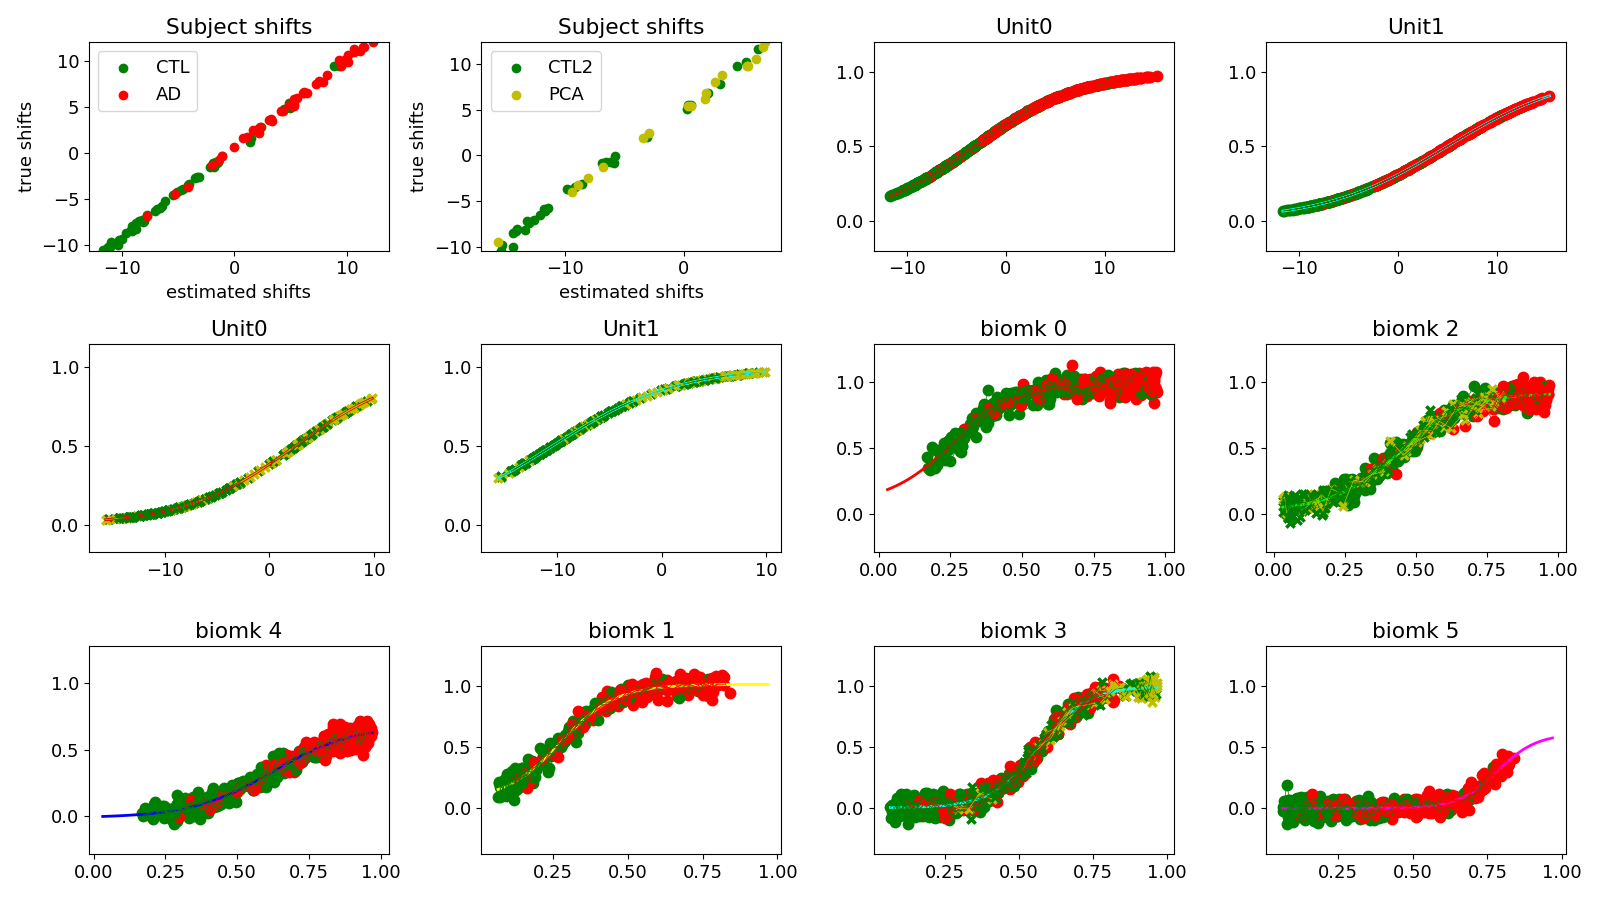
\includegraphics[width=\textwidth]{images/dkt/plotHierData611_synth1Pen5_JMD.png}
%  \caption{(top-left) (top-left) Scatter plots of the true shifts (y-axis) against estimated shifts (x-axis), for the 'synthetic AD' (left) and 'synthetic PCA' (right) diseases. (top-right and middle-left) Trajectories of unit }
%  \label{fig:dktSynthTrajHierData}
% \end{figure}

\begin{figure}
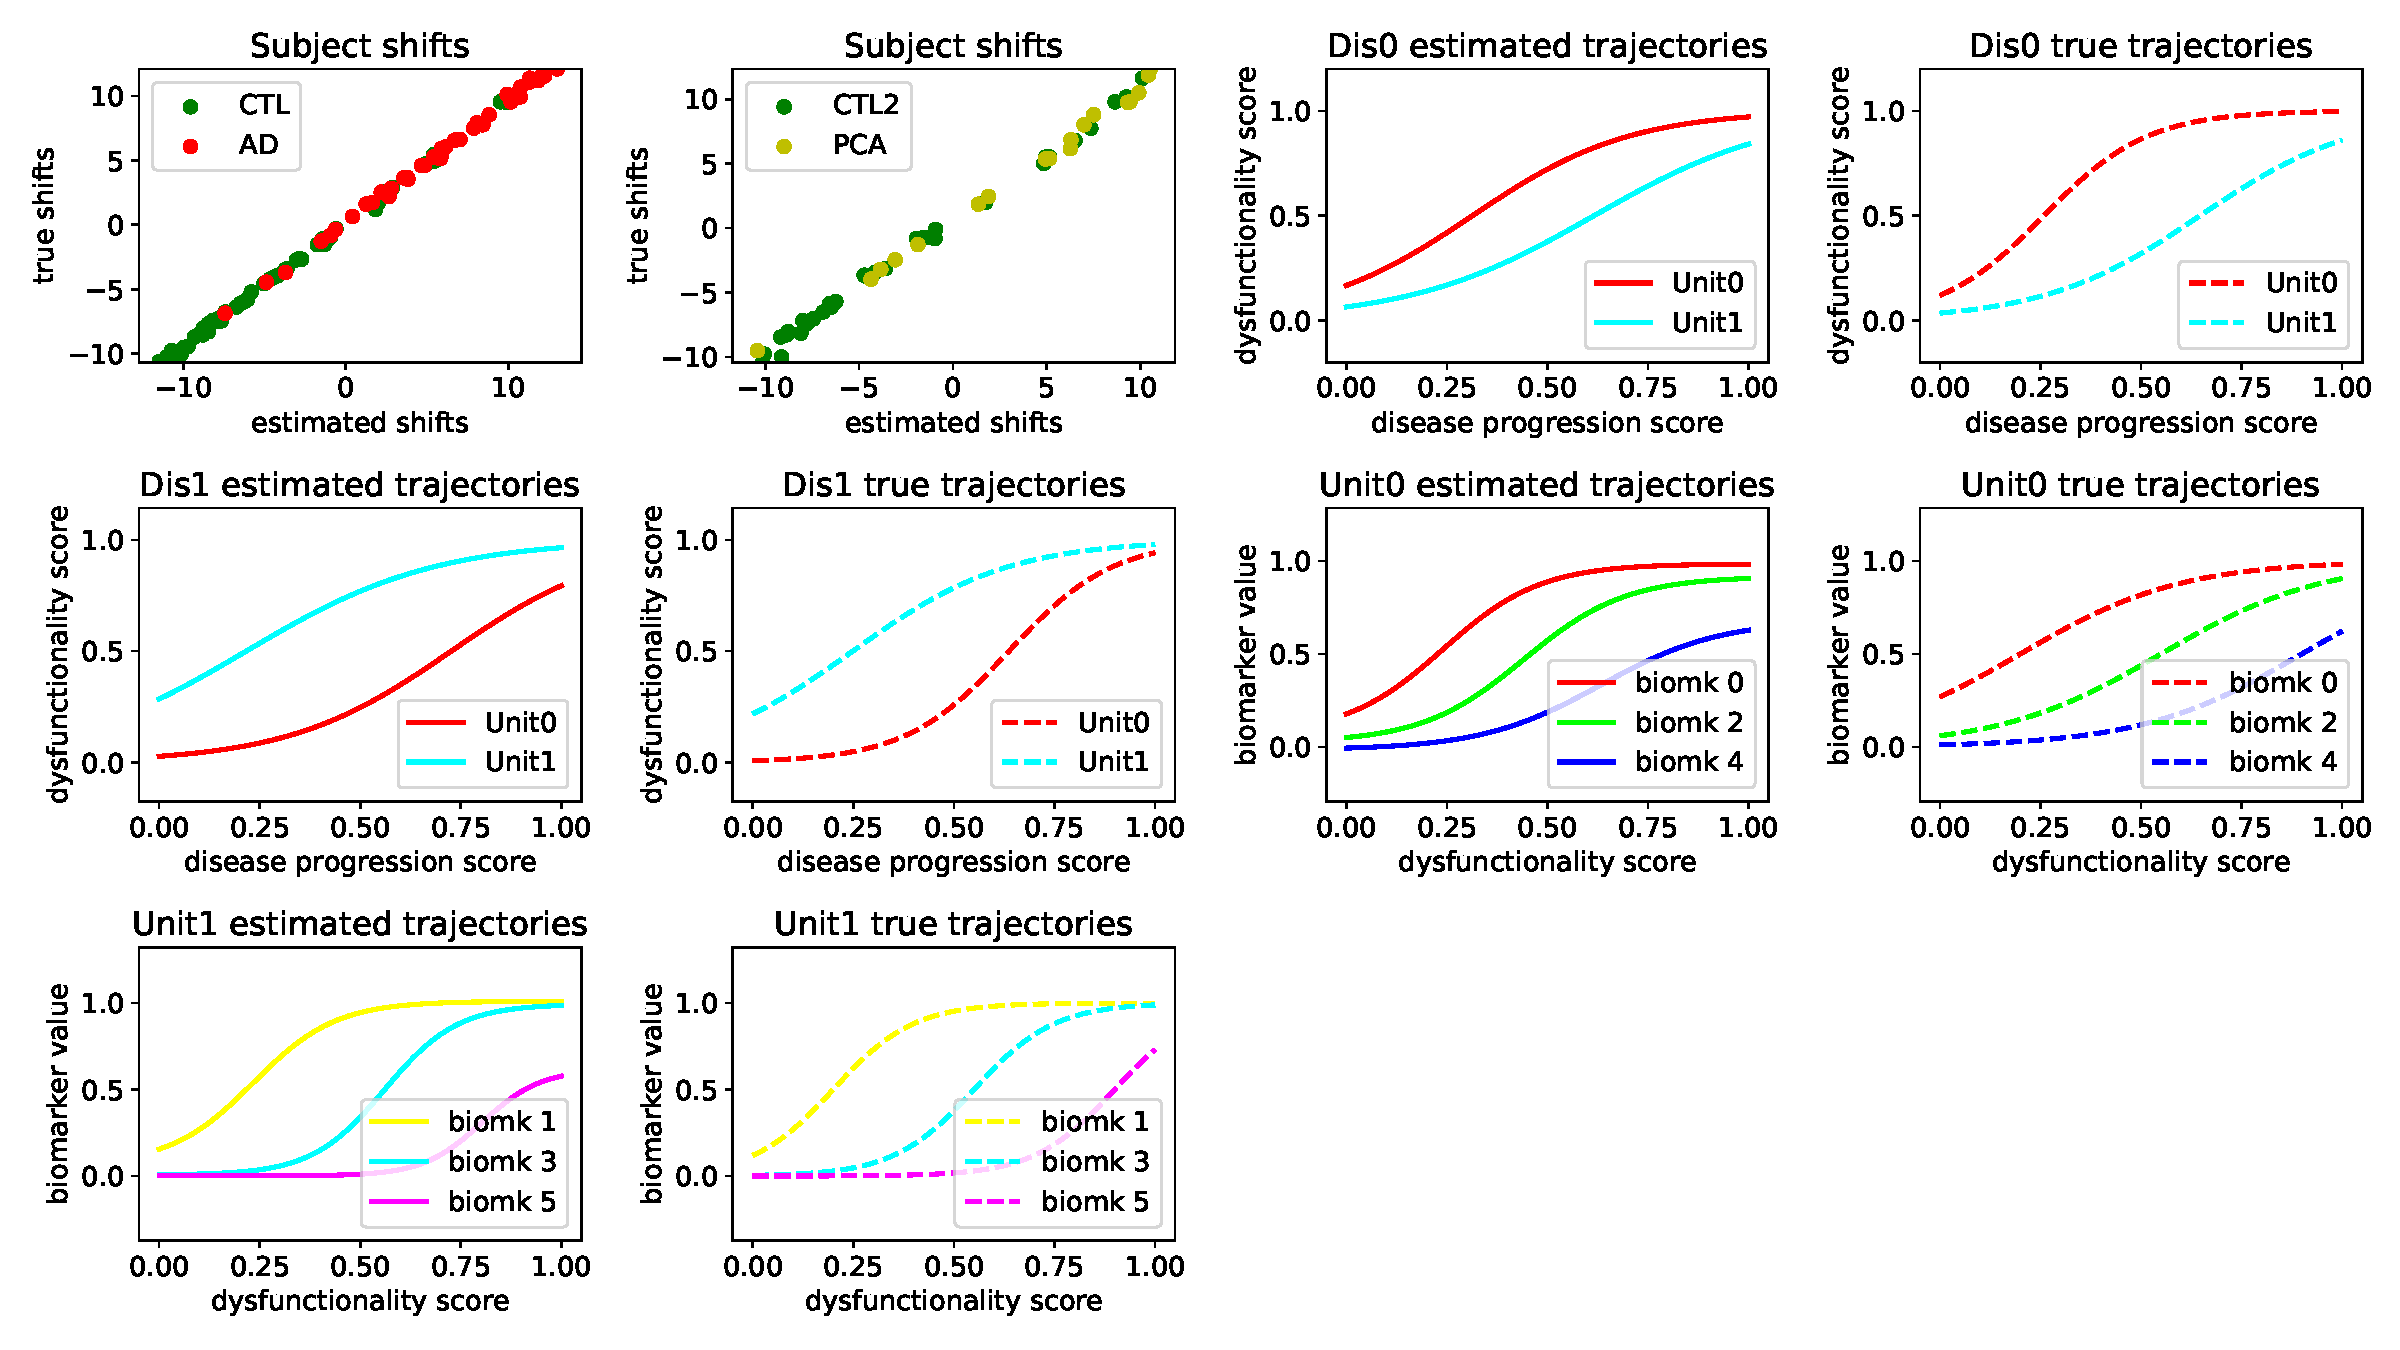
\includegraphics[width=\textwidth]{\jmdFld/resfiles/synth/synth1_JMD/compTrueParams101_synth1_JMD.pdf}
 \caption[DKT Simulation Results - Comparison between true and DKT-estimated biomarker trajectories and subject time-shifts.]{Comparison between true and DKT-estimated subject time-shifts and biomarker trajectories. (top-left) Scatter plots of the true shifts (y-axis) against estimated shifts (x-axis), for the 'synthetic AD' (left) and 'synthetic PCA' (right) diseases. We also show the DKT-estimated and true trajectories of the functional units within the 'synthetic AD' disease (top-right) and the 'synthetic PCA' disease (middle-left). For these figures, the x-axis measures the normalised disease progression score $s_i$ while the y-axis measures the dysfunctionality scores $f(s_i;\lambda_d^l)$. Finally, we also show the biomarker trajectories within unit 0 (middle-right) and unit 1 (bottom), where the x-axis represents the dysfunctionality scores $f(s_i;\lambda_d^l)$ and the y-axis represents the biomarker value.}
 \label{fig:dktSynthTrajCompTrue}
\end{figure}

\begin{figure}
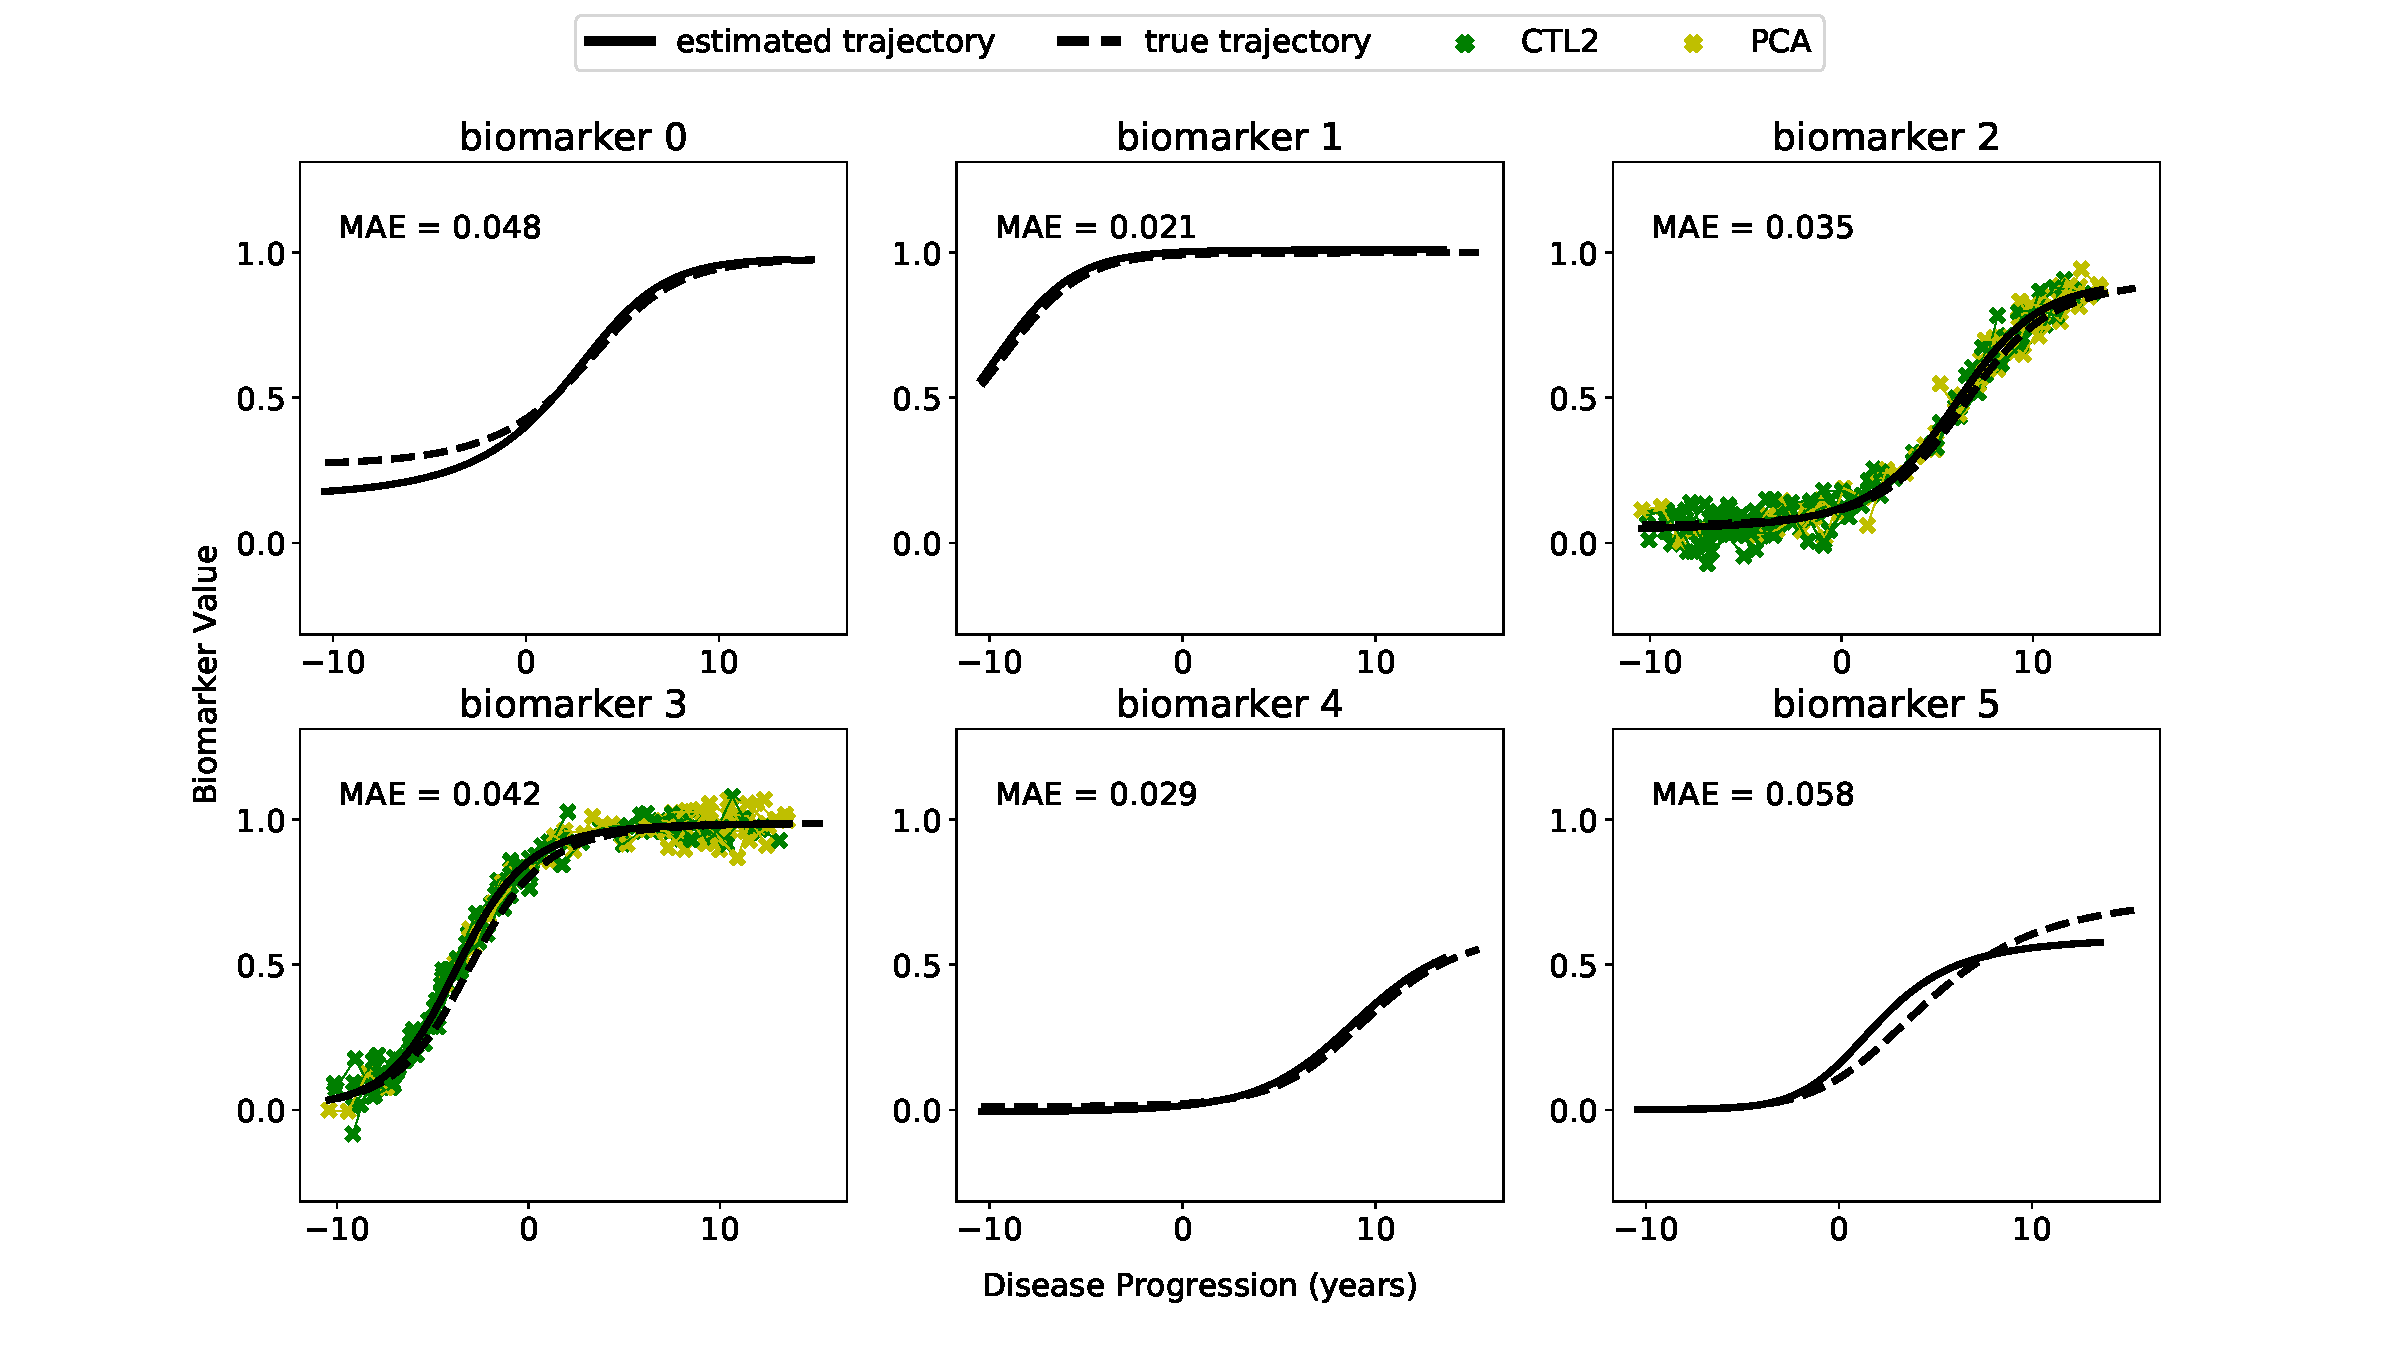
\includegraphics[width=\textwidth]{\jmdFld/resfiles/synth/synth1_JMD/trajDisSpaceDis1_101_synth1_JMD.pdf}
 \caption[Estimated biomarker trajectories for the "synthetic PCA" disease, plotted alongside true trajectories]{Estimated biomarker trajectories for the "synthetic PCA" disease, plotted alongside true trajectories. Estimation of the trajectories in biomarkers 0,1,4 and 5 has been done without any data from the "synthetic PCA" disease, only based on the disease-agnostic correlations with biomarkers 2 and 3.}
 \label{fig:dktSynthTrajDrcSpace}
\end{figure}


\subsection{Results on TADPOLE and DRC Datasets}
\label{sec:dktResTadDrc}

% Fig1: biomarker traj. over dysfunction scores in one functional unit -> Fig2: dysfunction trajectories over disease stage in the two disease models -> Fig3: inferred biomarker trajectories "directly" over disease stage  in PCA
Fig. \ref{fig:dktFitUnit} shows the estimated biomarker trajectories within the \emph{occipital unit} plotted over the dysfunction scores, along with samples from the model posterior and aligned subject data. The X-axis shows the dysfunctionality scores within the occipital unit, which represent estimated time-shifts, in months, from an arbitrary reference X=0, while the Y-axis shows biomarker values normalised to [0,1] range. The model shows an unbiased data fit (Fig. \ref{fig:dktFitUnit}), and we can observe most PCA subjects having abnormal occipital volumes, thus leading to high occipital dysfunctionality scores, in line with the current understanding of PCA as affecting posterior regions \cite{crutch2012posterior}. We also show the progression of dysfunctionality scores over the disease stage for typical AD (Fig \ref{fig:dktFitAD}) and PCA (Fig \ref{fig:dktFitPCA}). In typical AD, we see that hippocampal dysfunction becomes abnormal earliest, while PCA shows early hippocampal dysfunction, which is later exceeded by the dysfunction in the occipital, temporal and parietal regions, which are known to be affected in PCA \cite{crutch2012posterior,Baron2001}. 

In Fig. \ref{fig:PCAtrajByModality}, we plot the inferred biomarker trajectories for PCA directly across the disease progression. We do this for five different modalities: MRI Volumes, DTI, FDG, AV45 and AV1451. The results again recapitulate known patterns in PCA, where posterior regions are predominantly affected in all modalities. However, for MRI volumes and AV45, we also see early abnormalities, which we attribute to the models underestimating the biomarker measurement noise.


\begin{figure}
\centering
\begin{subfigure}{\textwidth}
\centering
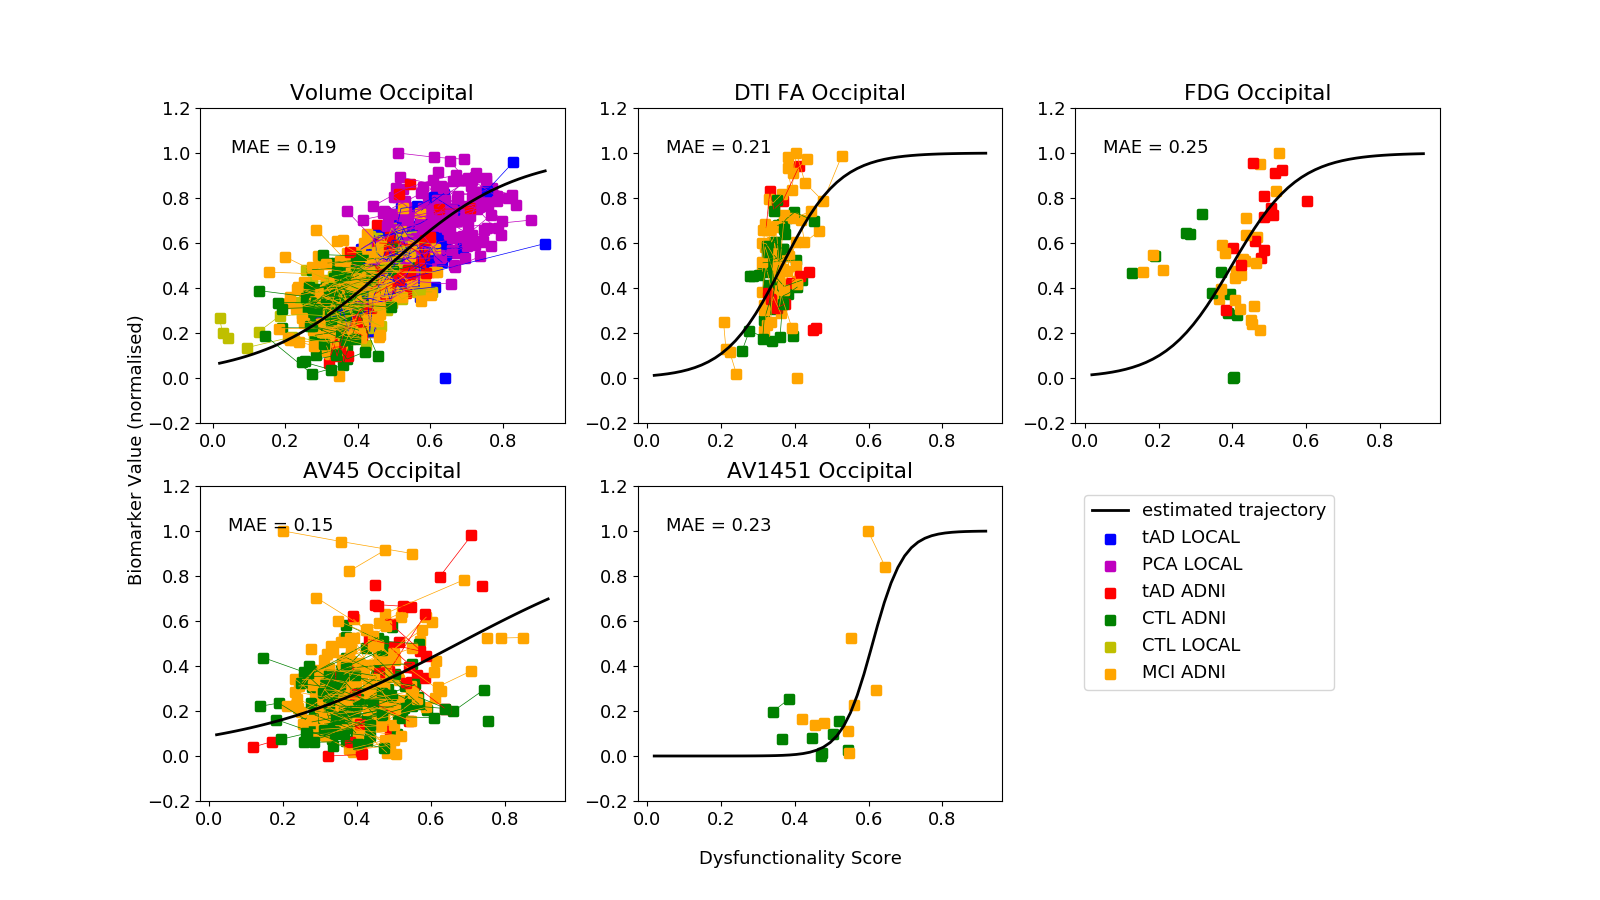
\includegraphics[width=1\textwidth, trim=90 20 110 0, clip]{\expFld/unit1_allTraj.png}
\caption{Occipital unit}
\label{fig:dktFitUnit}
\end{subfigure}
\vspace{2em}

\begin{subfigure}{0.47\textwidth}
\centering
% typical AD\\
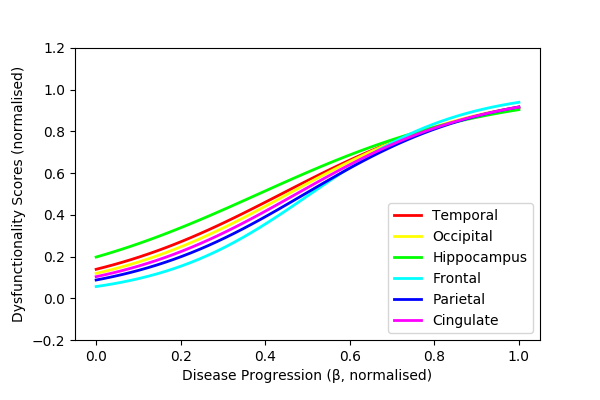
\includegraphics[width=1\textwidth, trim=0 0 0 20, clip]{\expFld/dis0_tAD_allTrajZeroOne.png}
\caption{tAD}
\label{fig:dktFitAD}
\end{subfigure}
\begin{subfigure}{0.47\textwidth}
\centering
% PCA\\
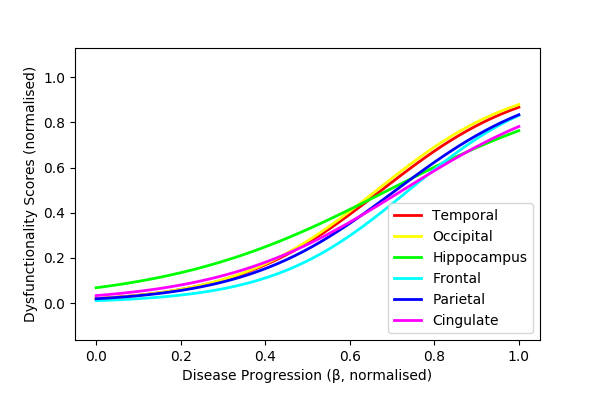
\includegraphics[width=1\textwidth, trim=0 0 0 20, clip]{\expFld/dis1_PCA_allTrajZeroOne.png}
\caption{PCA}
\label{fig:dktFitPCA}
\end{subfigure}
\caption[DKT results - biomarker trajectories in the occipital unit and dysfunctionality scores for tAD and PCA]{(a) DKT-estimated biomarker trajectories in the occipital functional unit. Subject data from ADNI and our local DRC cohort are also shown. The X-axis, defined as the occipital dysfunctionality score, represents the time-shifts (in months) of each subject. (b-c) Progression of DKT-estimated dysfunctionality scores for (b) typical AD and (c) PCA.}
\label{fig:pcaTadDisSpace}
\end{figure}

% estimated (hypothetical) trajectories in PCA: DTI, FDG, AV45, AV1451.Volumetric trajectories were based on PCA MRI data.
\begin{figure}
 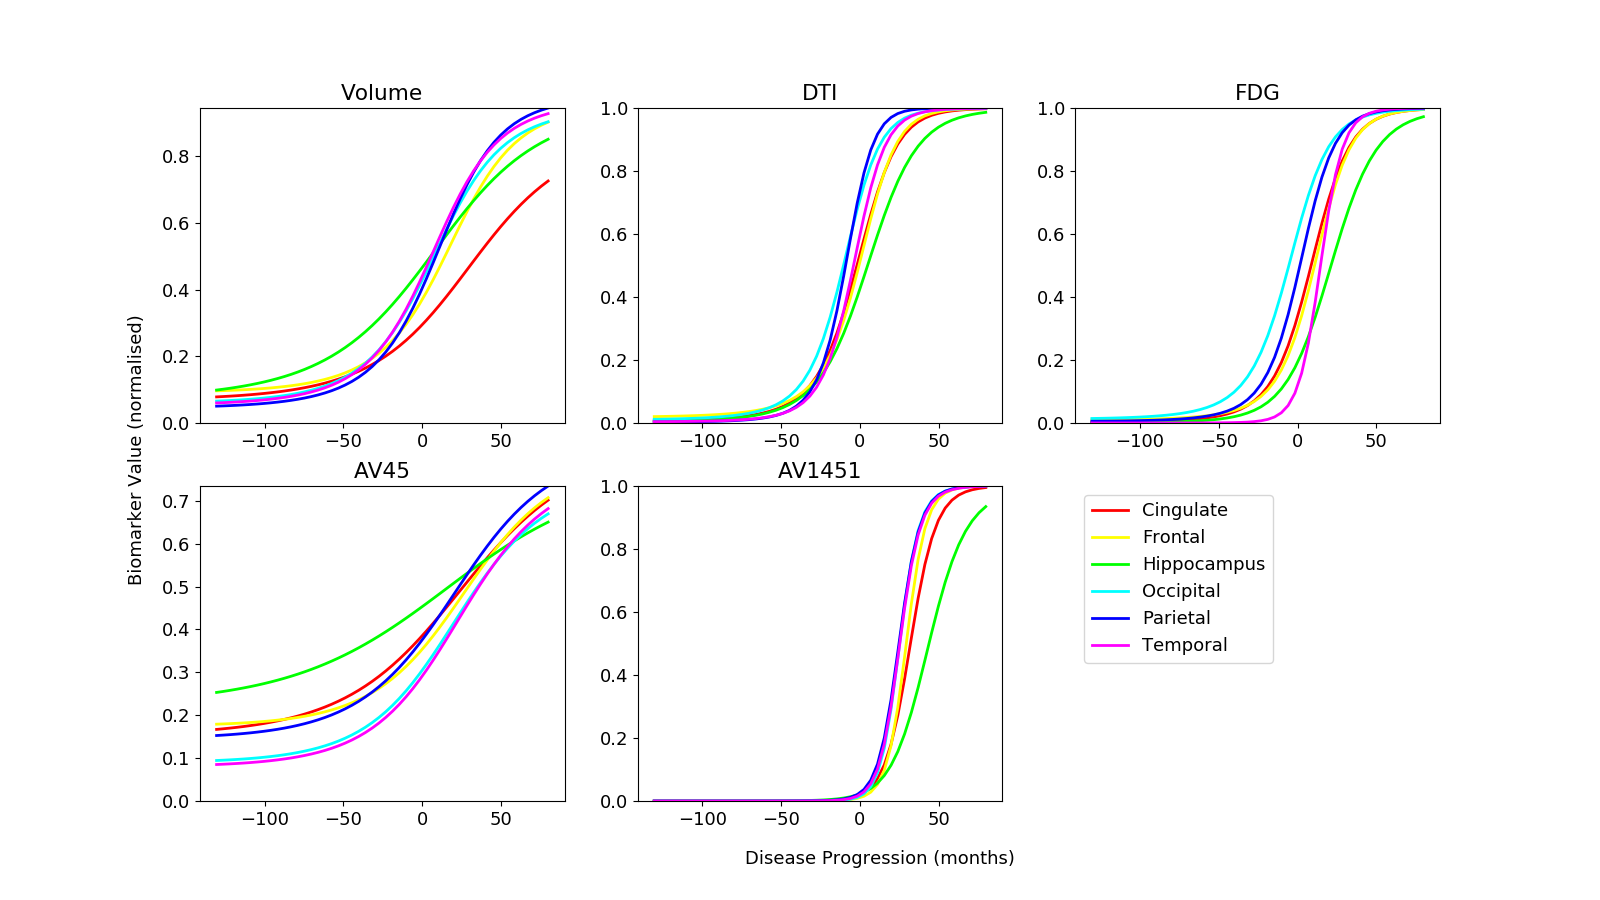
\includegraphics[width=\textwidth, trim=0 20 0 0, clip]{\expFld/trajDisSpaceOverlap_PCA_tad-drcTinyPen5_JMD.png}
 \caption[Estimated multi-modal trajectories for the PCA cohort.]{Estimated multi-modal trajectories for the PCA cohort. The only data that were available were the MRI volumetric data. The dynamics of the other biomarkers has been inferred by the model using data from typical AD, and taking into account the different spatial distribution of pathology in PCA as compared to typical AD.}
 \label{fig:PCAtrajByModality}
\end{figure}


\section{Validation on DTI Data in PCA}
\label{sec:dktResVal}

We further validated DKT by predicting unseen DTI data from two patient datasets:
\begin{itemize}
 \item TADPOLE subjects with a different progression from the training subjects
 \item A separate test set of 20 DTI scans from controls and PCA patients from our own cohort.
\end{itemize}

To split TADPOLE into subgroups with different progression, we used the SuStaIn model by \cite{young2018uncovering}, which resulted into three subgroups: hippocampal, cortical and subcortical, with prominent early atrophy in the hippocampus, cortical and subcortical regions respectively. To evaluate prediction accuracy, we computed the rank correlation between the DKT-predicted biomarker values and the measured values in the test data. We compute the rank correlation instead of mean squared error as it is not susceptible to systemic biases of the models when predicting "unseen data" in a certain disease. We also compared the performance of DKT at predicting unseen data with four other models: 
\begin{itemize}
 \item \emph{Latent stage model}: a sigmoidal based disease progression model, as described in \cite{jedynak2012computational}. This model assumes all tAD and PCA subjects follow the same progression.
 \item \emph{Multivariate}: A multivariate Gaussian Process model with RBF kernel that predicts a DTI ROI marker from multiple MRI markers.
 \item \emph{Spline}: a univariate cubic spline regression model that predicts the DTI biomarker based on the corresponding MRI biomarker, independently for each region.
 \item \emph{Linear}: Same as above but linear model instead of spline.
\end{itemize}



Validation results are shown in Table \ref{sec:dktPerfMetrics}, for hippocampal to cortical TADPOLE subgroups, as well as PCA subjects from our DRC cohort. When predicting missing DTI markers from the TADPOLE cortical subgroup as well as PCA subjects, the DKT correlations are generally high for the cingulate, hippocampus and parietal, and lower for the frontal lobe. DKT further shows favourable performance compared to the other models, due to its ability to disentangle the progressions of each disease separately. In particular, it shows the best results for DTI FA prediction in the parietal and temporal lobes on both datasets and similar performance to the latent-stage model on the PCA dataset for the cingulate, frontal and hippocampal (differences here are not statistically significant). Due to the challenging problem of predicting unseen data in these diseases/subtypes, notice how the models yield bad predictions for the occipital lobe (negative correlations), most likely due to overfitting.


\newcommand{\cw}{c}

\begin{table}
\centering
\fontsize{9}{12}\selectfont
\begin{tabular}{c | c c c c c c}
\textbf{Model} & \textbf{Cingulate} & \textbf{Frontal} & \textbf{Hippocam.} & \textbf{Occipital} & \textbf{Parietal} & \textbf{Temporal}\\
& \multicolumn{6}{c}{\textbf{TADPOLE subgroups: Hippocampal subgroup to Cortical subgroup}}\\
DKT (ours) &      0.56 $\pm$ 0.23 &    \textbf{0.35 $\pm$ 0.17} &        \textbf{0.58 $\pm$ 0.14} &     -0.10 $\pm$ 0.29 &     \textbf{0.71 $\pm$ 0.11} &     \textbf{0.34 $\pm$ 0.26} \\
Latent stage &      0.44 $\pm$ 0.25 &    0.34 $\pm$ 0.21 &       0.34 $\pm$ 0.24* &     \textbf{-0.07 $\pm$ 0.22} &     0.64 $\pm$ 0.16 &    0.08 $\pm$ 0.24* \\
Multivariate &      \textbf{0.60 $\pm$ 0.18} &   0.11 $\pm$ 0.22* &       0.12 $\pm$ 0.29* &     -0.22 $\pm$ 0.22 &   -0.44 $\pm$ 0.14* &   -0.32 $\pm$ 0.29* \\
Spline &    -0.24 $\pm$ 0.25* &  -0.06 $\pm$ 0.27* &        0.58 $\pm$ 0.17 &     -0.16 $\pm$ 0.27 &    0.23 $\pm$ 0.25* &    0.10 $\pm$ 0.25* \\
Linear &    -0.24 $\pm$ 0.25* &   0.20 $\pm$ 0.25* &        0.58 $\pm$ 0.17 &     -0.16 $\pm$ 0.27 &    0.23 $\pm$ 0.25* &    0.13 $\pm$ 0.23* \\
& \multicolumn{6}{c}{\textbf{typical Alzheimer's to Posterior Cortical Atrophy}}\\
DKT (ours) &    0.77 $\pm$ 0.11 &    0.39 $\pm$ 0.26 &      0.75 $\pm$ 0.09 &    0.60 $\pm$ 0.14 &    \textbf{0.55 $\pm$ 0.24} &    \textbf{0.35 $\pm$ 0.22} \\
Latent stage &    \textbf{0.80 $\pm$ 0.09} &    \textbf{0.53 $\pm$ 0.17} &      \textbf{0.80 $\pm$ 0.12} &    0.56 $\pm$ 0.18 &    0.50 $\pm$ 0.21 &    0.32 $\pm$ 0.24 \\
Multivariate &   0.73 $\pm$ 0.09 &   0.45 $\pm$ 0.22  &    0.71 $\pm$ 0.08 & -0.28 $\pm$ 0.21* &  0.53 $\pm$ 0.22  &  0.25 $\pm$ 0.23* \\
Spline &   0.52 $\pm$ 0.20* &  -0.03 $\pm$ 0.35* &     0.66 $\pm$ 0.11* &   0.09 $\pm$ 0.25* &    0.53 $\pm$ 0.20 &   0.30 $\pm$ 0.21* \\
Linear &   0.52 $\pm$ 0.20* &    0.34 $\pm$ 0.27 &     0.66 $\pm$ 0.11* &    \textbf{0.64 $\pm$ 0.17} &    0.54 $\pm$ 0.22 &   0.30 $\pm$ 0.21* \\
\end{tabular}
\vspace{0.5em}
\caption[Performance evaluation of DKT and other models]{Performance evaluation of DKT and four other statistical models of decreasing complexity. We show the rank correlation between predicted biomarkers and measured biomarkers in (top) TADPOLE subgroups -- information transfer from hippocampal subgroup to cortical subgroup -- and (bottom) PCA. (*) Statistically significant difference in the performance of DKT vs the other models, based on a two-tailed t-test, Bonferroni corrected.}
% \end{footnotesize}
\label{sec:dktPerfMetrics}
\end{table}



\section{Discussion}
\label{sec:dktDis}


We presented DKT, a framework that enables, for the first time, joint modelling of biomarker progressions in multiple neurodegenerative diseases simultaneously. The framework allows the inference of biomarker trajectories in rare diseases, for which there is not enough data to allow estimation of such trajectories, and accounts for a different spatial distribution of pathology between distinct types of dementia. This further enables us to understand the complex mechanisms of rare diseases, as well as mechanisms shared between different types of related diseases.

We provided an example implementation of DKT using specific models of the biomarker trajectories, measurement noise and link function (the disease progression score). However, DKT should be considered as a general framework for joint modelling of biomarker trajectories within different diseases simultaneously. The actual implementation of DKT can thus be extended to use non-parametric trajectories, or more complex link functions that estimate not only subject time-shifts but also progression speed or higher order terms.

While in this work we have focused on Alzheimer's variants such as tAD and PCA, DKT can also be applied to other progressive neurodegenerative diseases of non-Alzheimer's type such as tauopathies (e.g. Frontotemporal dementia), synucleinopathies (e.g. Parkinson's disease), other neurodegenerative diseases such as Huntington's disease or Multiple Sclerosis, and even the normal ageing process. Cognitive tests can also be included in the disease-specific sub-models of DKT, or even allocated in the functional units of the regions that are responsible for those tasks, based on previous voxel-based morphometry studies. However, some care needs to be exercised when selecting the biomarkers and grouping them into functional units, as in some diseases the assumption of disease agnostic dynamics might not hold for some groups of molecular biomarkers. For example, some non-Alzheimer's tauopathies such as Frontotemporal dementia might show tau abnormalities but no corresponding amyloid abnormalities within the same region. In the case of Frontotemporal dementia, we recommend including higher-level biomarkers such as glucose metabolism from FDG, white matter degeneration from DTI or volume from structural MRI, but one should exclude amyloid markers. 

Our work has several limitations: 1) DKT assumes all subjects within a disease follow the same trajectory, without considering heterogeneity within the disease population, 2) the allocation of biomarkers into functional units has to be done using \emph{a-priori} human knowledge, 3) DKT currently works only on extracted brain features, discarding important information present in the brain morphometry, 4) for validation, the synthetic experiment we ran was limited to only one setting of the parameters and 5) the validation on patient data was also done only on a small set of 20 DTI scans, due to lack of multimodal data in PCA.

There are several potential avenues for further research: 1) to account for heterogeneity, DKT can also be easily extended to include subject-specific effects; 2) improved schemes for biomarker allocation to functional units can take connectivity into account, or derive it from the data automatically; 3) to account for brain morphometry and connectivity, DKT can be extended into a fully spatio-temporal model, by estimating continuous changes in volumetric brain images -- in this case, each voxel can have an associated dysfunctionality score that is derived from measurements of various modalities from that voxel; 4-5) DKT can be further validated on more complex synthetic experiments with variable parameter settings, and on patient data from ADNI, where the population could be \emph{a-priori} split into sub-groups with different progressions. On these subgroups, DKT can be used to transfer biomarker modalities that have been left out during training.



\section{Conclusion}
\label{sec:dktCon}

In this work I presented DKT, a novel method that can empower studies of rare dementias with limited biomarker data by leveraging data from larger datasets of related dementias. When applied to synthetic data with ground truth, I showed that DKT can robustly recover biomarker trajectories in two distinct diseases and also subject-specific time-shifts. I also applied DKT to multimodal imaging biomarkers from the TADPOLE Challenge dataset, where I showed that it can estimate plausible non-MRI biomarker trajectories for Posterior Cortical Atrophy in lack of such data for this disease. I validated the performance of DKT on a test set of 20 DTI scans from PCA and controls, and showed that DKT has similar or better performance compared to simpler models.

In the next chapter, I will present the TADPOLE  Challenge, which evaluates the performance of algorithms and features at predicting the future evolution of subjects at risk of AD. As opposed to the work performed in this chapter, the TADPOLE challenge aims to evaluate a much larger set of algorithms and features, comprising regression techniques, disease progression models, machine learning techniques and even manual predictions made by clinicians.
